%%
%% Author: thompson
%% 03.11.17
%%

% Preamble
\documentclass[11pt]{article}

% Packages
\usepackage{a4wide}
\usepackage[utf8]{inputenc}
\usepackage[ngerman]{babel}
\usepackage{verbatim}
\usepackage{graphicx}
\usepackage{scrextend}

% Document
\begin{document}
    \section{Wireshark}
    \subsection{Setting up Wireshark}
    Für Ubuntu-Users funktioniert dies recht schnell.
    Im Terminal (Strg+Alt+T):
    \begin{verbatim}
    sudo apt-get install wireshark
    ...
    sudo dpkg-reconfigure wireshark-common
    sudo adduser 'whoami' wireshark
    \end{verbatim}
    Sollte weiterhin kein mitschneiden möglich sein, da der Zugriff auf /usr/bin/dumpcap nicht gestattet wird, so folgt:
    \begin{verbatim}
    sudo chmod +x /usr/bin/dumpcap
    \end{verbatim}
    Wireshark wird anschließend über die Apllikationen oder über das Terminal ausgeführt, mithilfe des Befehls
    \begin{verbatim}
    wireshark
    \end{verbatim}
\pagebreak
    \subsection{Funktionalitäten von Wireshark}
    \subsubsection{Grundfunktionalitäten}
    Wireshark beobachtet stets die eingehenden Packete des jeweiligen Interfaces.
    Auf dessen Hauptseite kann man bereits die Internetschnittstellen des jeweiligen Gerätes erfassen und beobachten.

    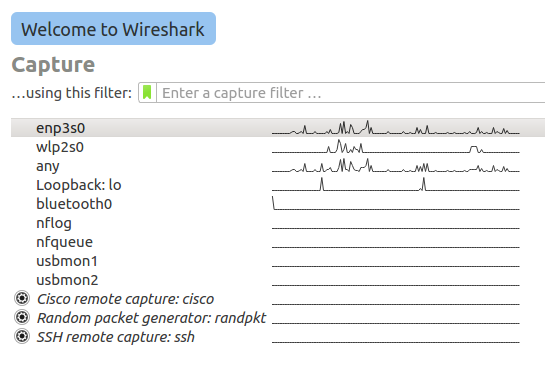
\includegraphics[width=\textwidth]{WiresharkMain.png}

    Möchte man ein gewisses Interface 'sniffen', so selektiert man dieses und startet die Beobachtung.

    \noindent\makebox[\textwidth]{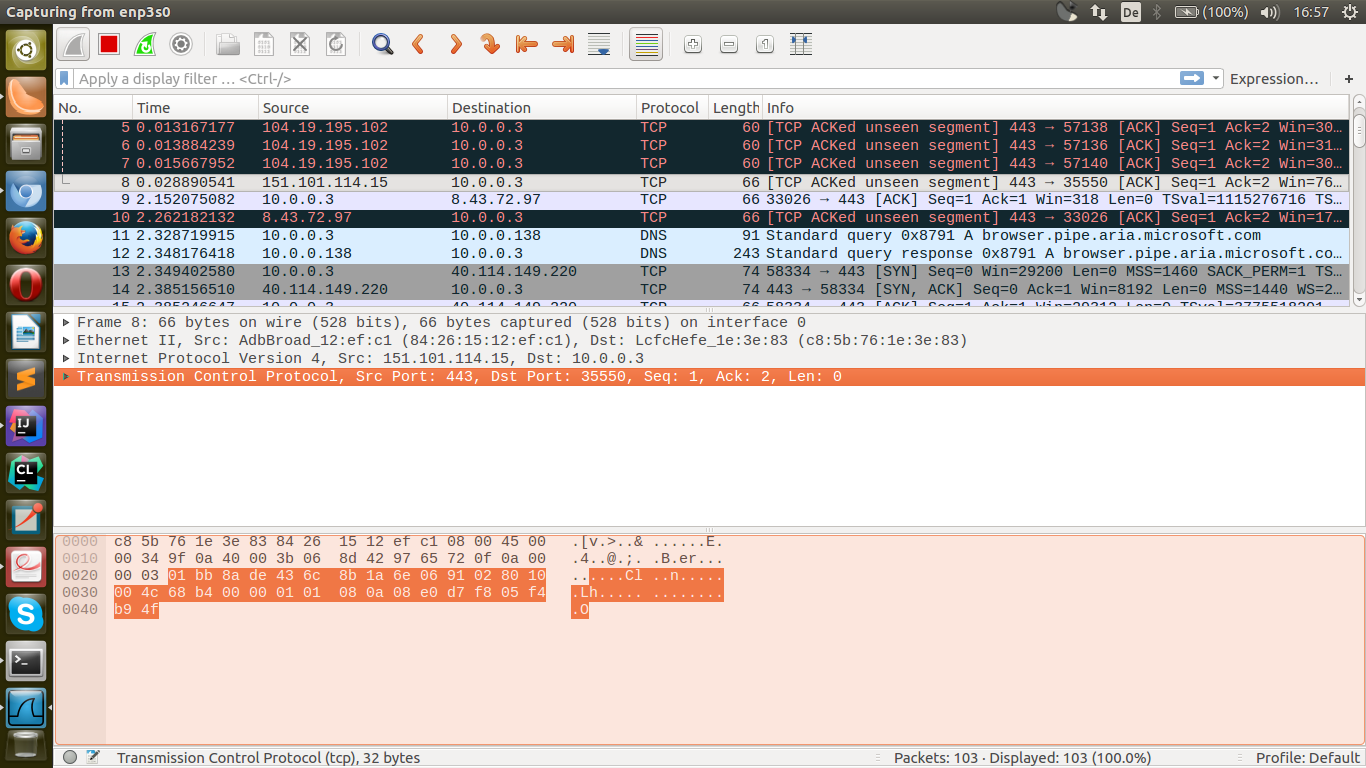
\includegraphics[width=\paperwidth]{WireSharkSniffing.png}}

    Hier beobachtet man eine explizite Schnittstelle zum Internet, mit all dessen Datatransfer.
    Ist der 'promiscuous mode' aktiviert, so erfasst man alle Packete die sich im derzeitigen Netzwerk bewegen, nicht nur des eigenen Gerätes.
\begin{verbatim}
    Capture > Options > verify "Enable promiscuous mode on all interfaces" checkbox
\end{verbatim}
    Im oberen Feld sieht man die eingehenden Packete, mitsamt
    \begin{addmargin}[1em]{1em}
        - Packetnummer (Frame), seit Start\\
        - Dauer der Übertragung\\
        - Ursprungs-IP des Packetes\\
        - Ziel des Packetes\\
        - Das genutzte Protokol der Übertragung (DHCP, ARPA, TCP,...)\\
        - Die Länge das Packetes in Hexadezimalziffern\\
        - Informationen zum Packet, etwa der Request ein\\
    \end{addmargin}
    Die Färbungen deuten auf die Packetformate hin. Beispielsweise ist per default TCP pink oder UDP blau markiert. Schwarz gekennzeichnete Packete deuten auf
    Packete mit Fehlern hin.
    Für mehr, siehe
    \begin{verbatim}
        View > Coloring Rules
    \end{verbatim}

    Im mittleren Feld stehen konkrete Daten zum betrachteten Packet.
    Für gewöhnlich gliedert sich dieser Teil in
    \begin{addmargin}[1em]{1em}
        - Frame-Nummer und abgefangenen Bits\\
        ... mitsamt Daten über dieses Frame: Protocols in Frame, Marked, Ignored, ...\\\\
        - Verbindungstyp der Übertragung\\
        ... inklusive Sender-IP und Empfänger-IP, oftmals in IPv6-Format sowie Übertragungsprotokoll\\\\
        - und unterschiedlichen Informationen, je nach Protokollierungstyp.\\
        ... für TCP beispielsweise die Internet Protokol Version und das Transmission Control Protokol, inklusive deren Daten.\\\\
    \end{addmargin}

    Im unteren Feld steht dann der Inhalt der jeweiligen Frames in non-human readable Format.

    Eine weitere Interessante Funktion die WireShark bietet ist das direkte Verfolgen einer *-verbindung. Via
    \begin{verbatim}
        > Rightclick on Frame > Follow > *-Stream
    \end{verbatim}
    Lässt sich direkt untersuchen was im Rahmen einer Verbindung ausgetauscht wird.

    \noindent\makebox[\textwidth]{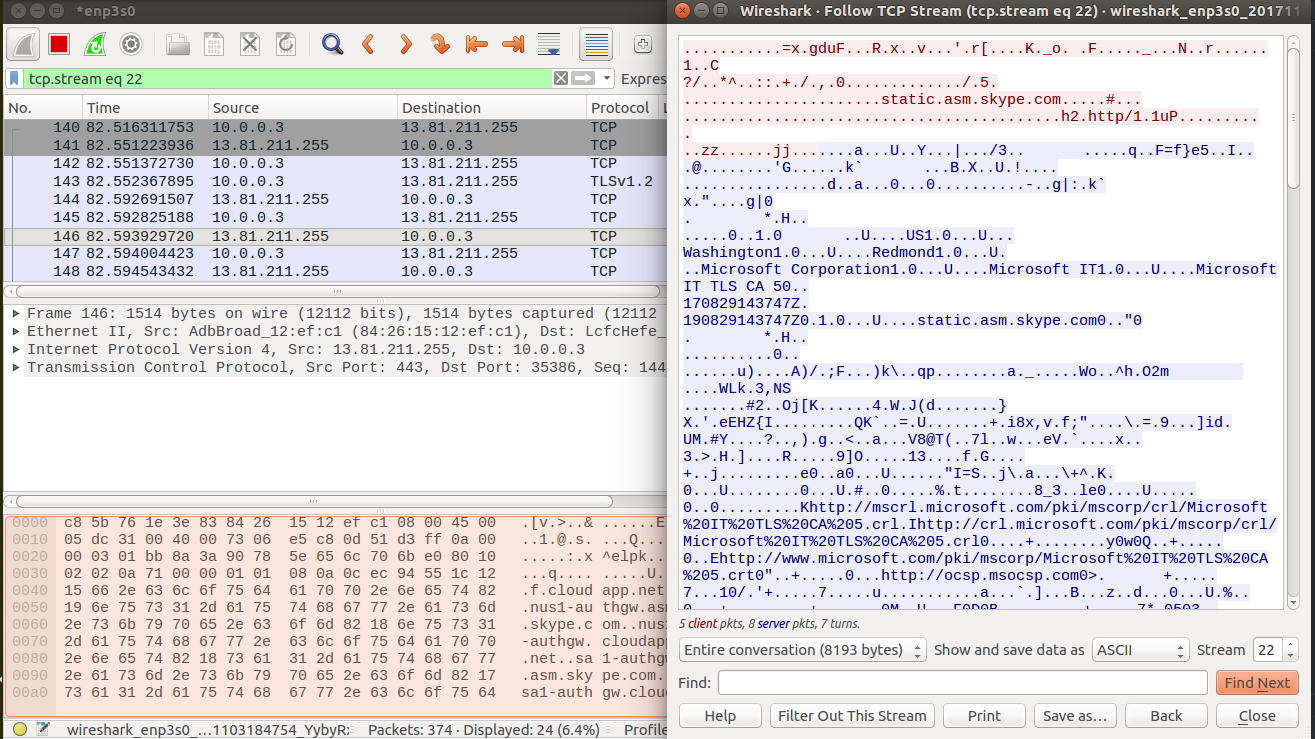
\includegraphics[width=\paperwidth]{WireSharkFollowTCPStream.png}}

    \subsubsection{Filtering}
    Um etwas spezifisches zu untersuchen, bietet WireShark Filteroptionen an.
    So kann man beispielsweise mit 'dns' explizit die DNS-Packete aus dem ganzen Satz an Packeten herausfiltern.
    Für weitere Optionen, siehe
    \begin{verbatim}
        Analyze > Display Filters
    \end{verbatim}
    Man kann auch eigene Filter erstellen und einbauen.\footnote[1]{$https://www.wireshark.org/docs/wsug\_html\_chunked/ChWorkBuildDisplayFilterSection.html$}\\
    Übliche Befehlskonfigurationen können wie folgt lauten:
    \begin{addmargin}[1em]{1em}
        $\diamond$ tcp.port==80\\
            -- Suche nach allen TCP verbindungen die an Port 80 docken\\
        $\diamond$ udp contains 64\\
            -- Suche durch alle Packete welche eine x64 Zahl im Frame aufweisen\\
        $\diamond$ http.connection matches "Keep-Alive"\\
            -- Suche nach allen TCP-Verbindungen mit Keep-Alive Kondition\\
        $\diamond$ tcp.flags \& 0x02 \\
            -- Suche durch alle TCPs mit gesetzter SYNchronize-Flag\\
        $\diamond$ tcp.port in {80 443 8080}\\
            -- Suche alle TCPs welche an Port 80 oder 443 oder 8080 docken\\
    \end{addmargin}

    \subsubsection{Aufzeichnen von Datenverkehr}
    Das Aufzeichnen des Datenverkehrs erfolgt gewöhnlicherweise direkt mit dem Starten des Sniffings .
    % // TODO: More to add here? Not sure how to sniff on multiple streams

    Der 'promiscuous mode', wie oben bereits erwähnt, betrachtet auch Packete die an das jeweilige Netzwerk gesendet werden.

    Die Aufzeichnungen im 'promiscuous mode' sind in der Regel ungefährlich für alle Beteiligten, da Packete nur empfangen werden wenn sie
    tatsächlich der Empfänger-IP entsprechen. Jedoch kann man dies mit einem SPAN port, einem Switch Port Analyzer, umgehen, wodurch
    jegliche Packete durch das Gerät empfangen werden.\footnote[2]{https://blog.packet-foo.com/2016/07/how-to-use-wireshark-to-steal-passwords/}
    Aufgrund der Human-Readable-Umschreibung von betrachteten Streams, kann man somit sensible Daten wie Passwörter und IDs abfangen und auslesen.
    Eine Gegenmaßnahmen dazu sind Enkryptionen durch SSL oder TLS oder eingeschränkte Zutrittsrechte zu Serverräumen.\footnote[3]{https://blog.packet-foo.com/2016/11/the-network-capture-playbook-part-4-span-port-in-depth/}
    Um einen SPAN aufzusetzen benötigt man physikalischen Zugang zum jeweiligen Router.
\end{document}